\appendix

\section{Appendices}
\label{sec:appendix}

Included in this section are facts, figures, and tables that support our research but were not strictly required to communicate our findings effectively in the main paper body.

\subsection{BERT fine-tuning figures}

\vspace*{15pt}%

\begin{figure}[ht]
	\centering
	\begin{subfigure}{0.95\textwidth}%
		\centering
		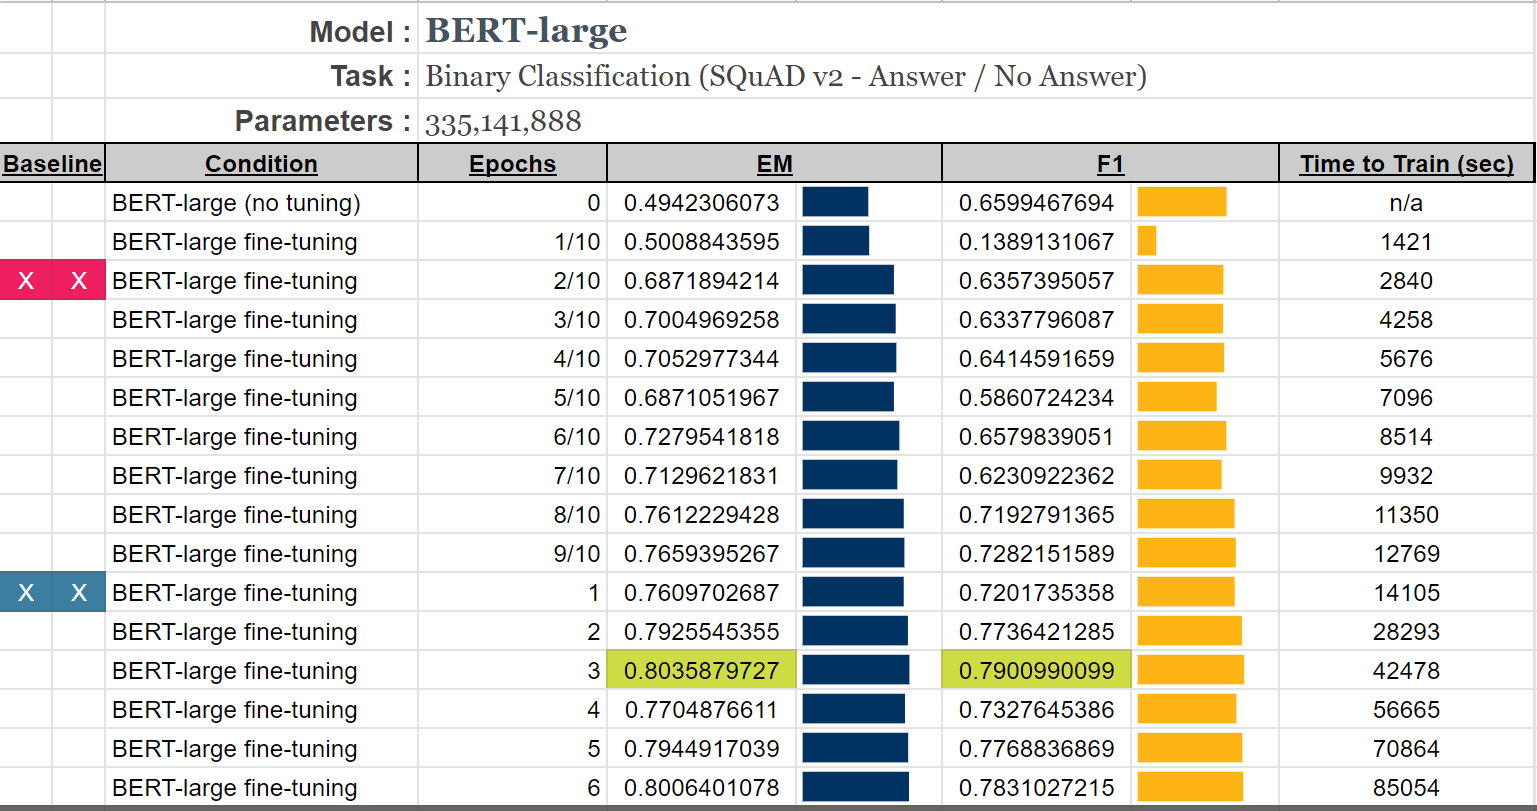
\includegraphics[width=\linewidth]{images/classification/BERT_Large_Training.png}%
		\caption{BERT$_{large}$ fine-tuning table : classification}
	\end{subfigure}%

	\vspace*{8pt}%
	
	\begin{subfigure}{0.96\textwidth}%
		\centering
		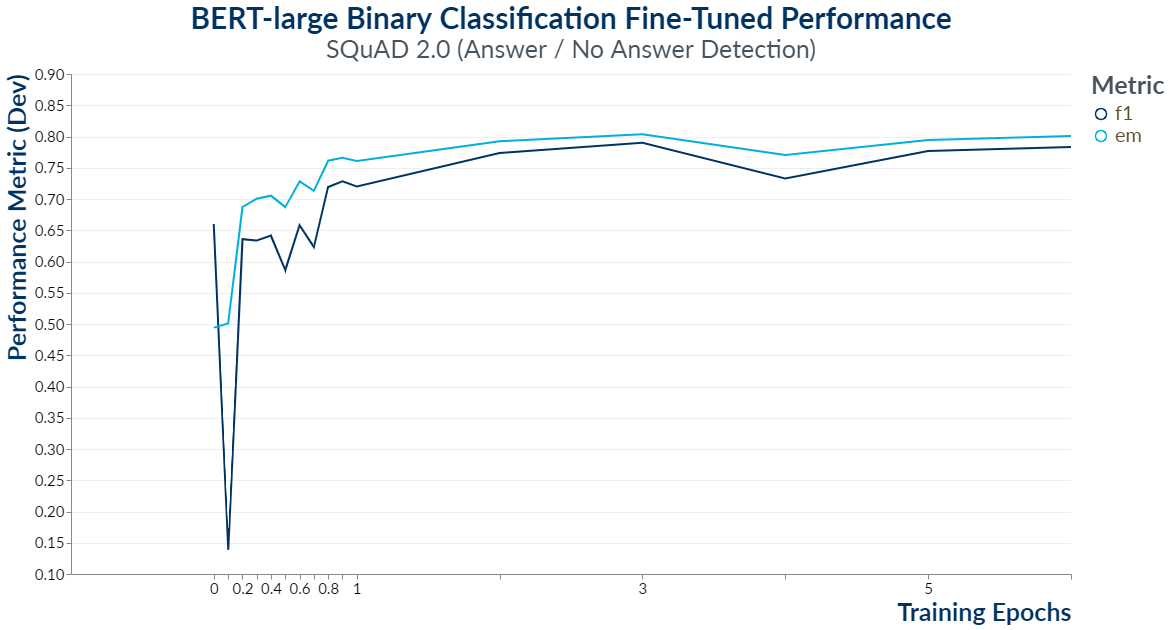
\includegraphics[width=\linewidth]{images/BinaryClassification_BERT_Training_Performance_plot.png}%
		\caption{BERT$_{large}$ fine-tuning plot : classification}
	\end{subfigure}%
	\caption{\label{apdx:BERT_fine_tuning_classification}BERT$_{large}$ fine-tuning for classification}
\end{figure}

\begin{figure}[ht]
	\centering
	\begin{subfigure}{0.95\textwidth}%
		\centering
		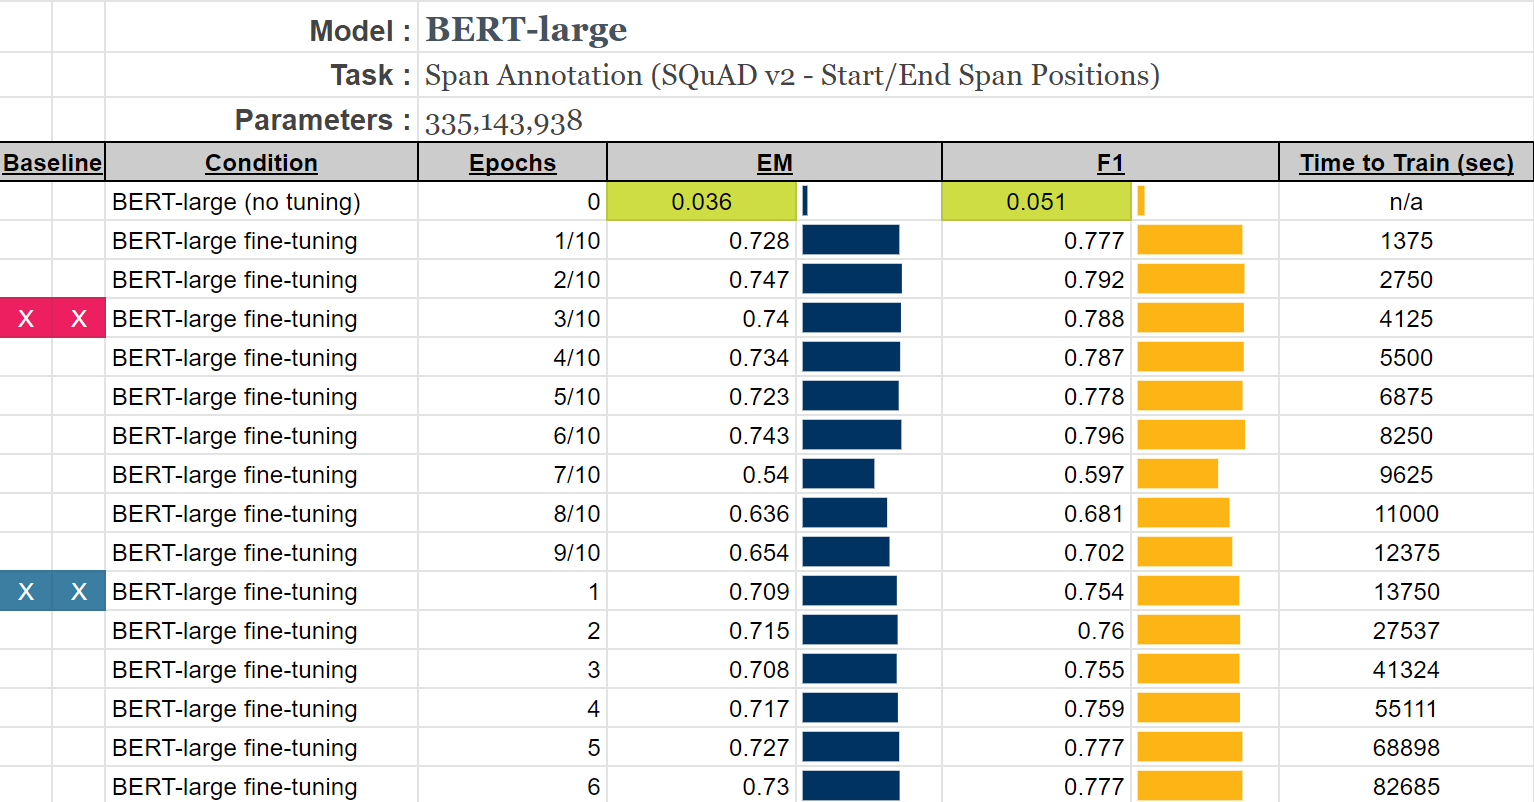
\includegraphics[width=\linewidth]{images/span/BERT_Large_Training.png}%
		\caption{BERT$_{large}$ fine-tuning table : span annotation}
	\end{subfigure}%
	
	\vspace*{8pt}%

	\begin{subfigure}{0.96\textwidth}%
		\centering
		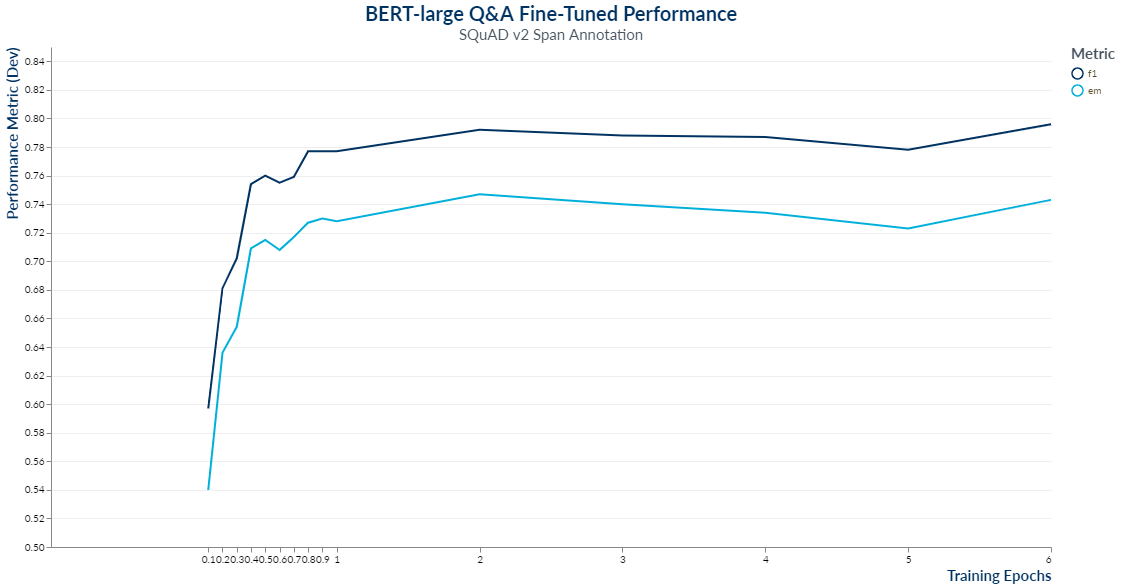
\includegraphics[width=\linewidth]{images/QnA_BERT_Training_Performance_plot.png}%
		\caption{BERT$_{large}$ fine-tuning plot : span annotation}
	\end{subfigure}%
	\caption{\label{apdx:BERT_fine_tuning_span_annotation}BERT$_{large}$ fine-tuning for span annotation}
\end{figure}
